\newpage
\section{Peugeot Infotainment sustav}\label{sec:van_bus}

\subsection{Principi i fizikalne zakonitosti}
VAN (eng. \textit{Vehicle Area Network}) je serijska komunikacijska sabirnica koju su razvili PSA grupa (Peugeot, Citroën) i Renault kao alternativu CAN sabirnici. 
Definirana je u ISO standardu \textbf{ISO 11519-3}. 
Koristi isti fizički sloj kao CAN sabirnica (diferencijalni par) i identičnu metodu arbitraže na sabirnici, 
ali se razlikuje u načinu pakiranja podataka.
Gotovo sve informacije navedene ovdje preuzete su iz Atmel TSS463C dokumentacije \cite{tss463c_datasheet}.

\bigskip
\noindent
Kao i CAN, VAN protokol koristi identifikatore za razlikovanje poruka i izvođenje arbitraže na sabirnici. 
Dodatno, omogućuje tzv. „odgovore unutar okvira” (eng. \textit{In-frame}), veće veličine poruka (28 bajtova umjesto 8 bajtova kao u CAN-u) 
te mogućnost izravne komunikacije s drugim uređajem.

\bigskip
\noindent
Podaci na VAN mreži pakiraju se u okvire. 
Okviri se sastoje od više dijelova: početka okvira (\textbf{SOF}), identifikatora poruke (\textbf{IDEN}), 
naredbe (\textbf{COM}), samih podataka (\textbf{DATA}), kontrolnog zbroja okvira (\textbf{FCS}), 
signala kraja podataka (\textbf{EOD}), signala potvrde (\textbf{ACK}) te signala kraja okvira (\textbf{EOF}).

\begin{table}[H]
    \centering
    \fontsize{10}{10}
    \selectfont
    \begin{tabular}{|c|c|c|c|c|c|c|c|c|c|c|}
        \hline
        \multirow{2}{*}{\makecell{SOF             \\ 10 TS}}  & \multirow{2}{*}{\makecell{IDEN \\ 12 bit \\ 15 TS}} & \multicolumn{4}{c|}{\makecell{Command \\ (4 bit, 5 TS)}} & \multirow{2}{*}{\makecell{DATA max. \\ 28 byte \\ 280 TS}} & \multirow{2}{*}{\makecell{FCS \\ 15 bit \\ 18 TS}} & \multirow{2}{*}{\makecell{EOD \\ 2 TS}} & \multirow{2}{*}{\makecell{ACK \\ 2 TS}} & \multirow{2}{*}{\makecell{EOF \\ 4 TS}} \\[7mm] \cline{3-6}
         &  & EXT & RAK & R/W & RTR &  &  &  &  & \\
        \hline
    \end{tabular}
    \caption{Oblik VAN okvira}
    \label{fig:van_frame_format}
\end{table}

\subsubsection{e-Manchester kodiranje}

Svi VAN okviri kodirani su pomoću unaprijeđenog Manchesterovog kodiranja (eng. \textit{Enhanced Manchester, e-Manchester}).
Kod e-Manchestera, nakon slanja tri NRZ bita, četvrti bit šalje se kao Manchesterov bit.
Slanje podataka na ovaj način omogućuje lakšu sinkronizaciju na sabirnici. 
Ovo je predvidljivija metoda ubacivanja bitova (eng. \textit{bit-stuffing}) u usporedbi s metodom korištenom na CAN sabirnici.

\bigskip
\noindent
U Tablici \ref{fig:van_frame_format} prikazan je broj bitova za svaki dio okvira, kao i broj vremenskih intervala (eng. \textit{Time Slots}, TS). 
Budući da Manchester bit zahtijeva dva vremenska intervala za prijenos, četiri bita u nizu kodirana e-Manchester metodom prenose se u 3 + 2 vremenska intervala.

\begin{figure}[H]
    \centering
    
\includegraphics[width=0.75\textwidth]{images/mux1-eman.pdf}
    \caption[]{e-Mancherster kodiranje \cite{mux1}}
    \label{fig:manchester_bits_mux1}
\end{figure}

\begin{figure}
    \centering
    
\includegraphics[width=0.5\textwidth]{images/manchester_bits.pdf}
    \caption{NRZ i Manchester bitovi. \cite{tss463c_datasheet}}
    \label{fig:manchester_bits_tss463_docs}
\end{figure}

\subsubsection{Poruke}

Uređaj ili modul povezan na mrežu može biti jednog od tri tipa:
\begin{itemize}
  \item Autonomni modul - glavni uređaj sabirnice. Može slati \textbf{SOF} niz, započeti prijenos podataka i primati poruke.
  \item Modul sa sinkronim pristupom - ne može slati \textbf{SOF} niz, ali može započeti prijenos podataka i primati poruke.
  \item Podređeni modul (eng. \textit{Slave}) - može slati poruke samo pomoću odgovora unutar okvira (eng. \textit{in-frame}) i također može primati poruke.
\end{itemize}

\begin{figure}
  \begin{center}
    
\includegraphics[width=0.75\textwidth]{images/ranking.pdf}
    \caption{Vrste modula, \cite{tss463c_datasheet}}
  \end{center}
\end{figure}

\noindent
VAN protokol podržava više tipova poruka. Razlikuju se pomoću polja identifikatora (\textbf{IDEN}) i naredbe (\textbf{COM}). Identifikator je dug 12 bita i slijedi ga 4 bita naredbe. Zbog načina na koji funkcionira arbitraža na sabirnici, manji identifikator ima prednost na sabirnici. Dok je vrijednost identifikatora potpuno proizvoljna, bitovi naredbe su strogo definirani i određuju tip poruke koja će se poslati na sabirnici:

\begin{itemize}
  \item EXT - uvijek 1
  \item RAK - `\emph{Request Acknowledge}' (zahtjev za potvrdom). Ako je 1, primatelj mora potvrditi primitak poruke. Ako je 0, signal ACK se ne šalje.
  \item R/W - `\emph{Read/Write}' (čitanje/pisanje). Označava smjer podataka. Ako je 0, radi se o poruci za pisanje (`\emph{write}'), gdje uređaj šalje podatke namijenjene drugom uređaju. Ako je 1, radi se o poruci za čitanje („\emph{read}”), što podrazumijeva zahtjev za podacima i očekuje odgovor.
  \item RTR - `\emph{Remote Transmission Request}' (zahtjev za daljinskim prijenosom). Ako je 0, poruka sadrži podatke. Ako je 1, poruka ne sadrži podatke i implicira zahtjev za odgovor unutar okvira (in-frame response). Kombinacija R/W = 0 i RTR = 1 je zabranjena na sabirnici.
\end{itemize}

\subsubsection{Vrste poruka}
\label{subsec:message-types}

Ovdje ćemo navesti tipove okvira relevantne za ovaj projekt. Postoje i drugi, ali koristimo samo ove.

\smallskip
\noindent
Podsjetnik: Dominantno = 0, Recesivno = 1.

\paragraph{Normalni okvir}

Najjednostavniji tip okvira. Jedan modul šalje cijeli okvir s podacima, te može, ali ne mora, zatražiti potvrdu (ACK). 
U slučaju da se potvrda ne traži, poruka se tretira kao poruka za emitiranje (eng. \textit{broadcast}).

\begin{figure}[H]
    \centering
    
\includegraphics[width=\textwidth]{images/normalframe_ack.pdf}
    \caption{Prijenos normalnog okvira sa ACK, \cite{tss463c_datasheet}}
    \label{fig:normal_frame_ack}
\end{figure}

\begin{figure}[H]
    \centering
    
\includegraphics[width=\textwidth]{images/normalframe_noack.pdf}
    \caption{Prijenos normalnog okvira bez ACK, \cite{tss463c_datasheet}}
    \label{fig:normal_frame_noack}
\end{figure}

\paragraph{Zahtjev sa trenutnim odgovorom}
\label{p:immediate-reply}

Ovo je jedini okvir u kojem podređeni modul (eng. \textit{slave}) može slati podatke. 
Jedina razlika na sabirnici je promjena stanja bita R/W u odnosu na normalni okvir.
Glavni modul sabirnice (eng. \textit{bus master}) generira \textbf{SOF}, inicijator generira identifikator i prva tri bita naredbe, te signal ACK. 
Ostalo (RTR, podaci i kontrolnu sumu) generira modul koji odgovara.

\begin{figure}[H]
\centering

\includegraphics[width=\textwidth]{images/immediate_reply.pdf}
\caption{Ilustracija prijenosa zahtjeva sa trenutnim odgovorom, \cite{tss463c_datasheet}}
\label{fig:immediate_reply_frame}
\end{figure}

\subsubsection{VAN mreža}

Više modula možemo povezati zajedno kako bismo stvorili mrežu. 
Također je moguće povezati više mreža i koristiti pristupni modul (eng. \textit{gateway}) za usmjeravanje podataka između mreža. 
U vozilu Peugeot 206 imamo jednu CAN mrežu \emph{CAN Engine} i tri VAN mreže: \emph{VAN Comfort}, \emph{VAN Body 1} i \emph{VAN Body 2}.

\noindent
Raspored mreža prikazan je na slici \ref{fig:van_can_network}. Tamo također možemo vidjeti pristupni modul, BSI. Ovaj modul prisutan je u svim vozilima PSA grupe. 
Konkretni BSI dolazi iz generacije AEE2001, jedine generacije koja koristi VAN sabirnicu. Druge generacije, AEE2004 i AEE2010, koriste isključivo CAN.
Naš infotainment sustav bit će spojen umjesto CD mjenjača, modul broj 8415 na slici \ref{fig:van_can_network} na \emph{VAN Comfort} sabirnici.

\begin{figure}[H]
  \begin{center}
    
\includegraphics[width=0.75\textwidth]{images/vannetwork.pdf}
    \caption{Pregled VAN i CAN mreže u Peugeot 206 automobilu \cite{sedre}}
    \label{fig:van_can_network}
  \end{center}
\end{figure}

Na slici \ref{fig:block_diagram_2_1} je prikazan block dijagram idejnog rješenja iz kojeg se mogu prepoznati tri dijela, kao i dio koji je centralni za ovaj projekt. Mikroupravljač je zadužen i za komunikaciju s računalom automobila, obradu dobivenih informacija te za njihov prikaz na ekranu.

\begin{figure}[H]
  \begin{center}
    
\includegraphics[width=0.75\textwidth]{images/block_diagram_2_1.pdf}
    \caption{Block dijagram idejnog rješenja}
    \label{fig:block_diagram_2_1}
  \end{center}
\end{figure}

\subsection{Pregled sklopovskog rješenja}

Na slici \ref{fig:block_diagram_2_2} se nalazi prikaz osnovnog sklopovskog dijagrama sustava. Glavni dio sustava je mikroupravljač koji ima ulogu komunikacije informacija s računalom automobila te obradu i prikaz tih istih informacija na ekranu. Kako mikroupravljač ne podržava VAN protokol, potrebno je koristiti upravljačke integrirane krugove koji pružaju sučelje s protokolom koji je podržan od strane mikroupravljača. Za slučaj da se ne pronađe upravljač koji ne podržava diferencijalni VAN protokol, bit će potrebno koristiti tzv. VAN Transciever kako bi preveli TTL logiku u diferencijalni par. Također zbog dodatne funkcionalnosti prikaza vremena na ekranu, potrebno je dodati RTC integrirani krug čija je zadaća praćenje stvarnog vremena te komunikacija istog s mikroupravljačem.

\begin{figure}[H]
  \begin{center}
    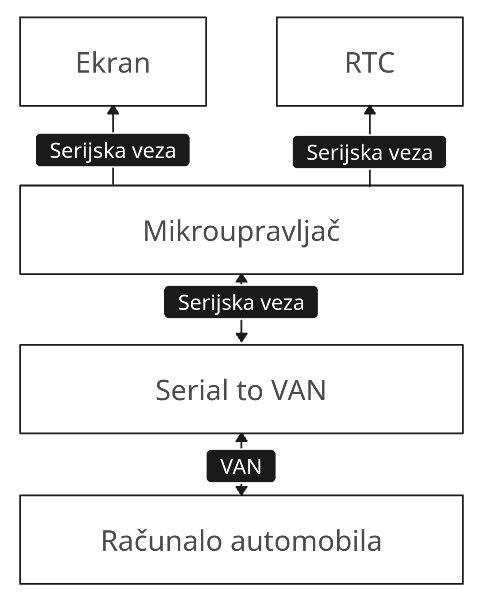
\includegraphics[width=0.75\textwidth]{images/block_diagram_2_2.png}
    \caption{Osnovni blok dijagram sklopovskog rješenja}
    \label{fig:block_diagram_2_2}
  \end{center}
\end{figure}

\subsection{Prijedlog programskog rješenja}
Na slici \ref{fig:block_diagram_2_3} je prikazan blok dijagram programskog rješenja koji daje abstraktan uvid u moguće programsko rješenje. Glavni program bi se vrtio na mikroupravljaču ESP32 koji je odgovaran za slanje i primanje paketa na VAN mreži tj. odgovaran je za komunikaciju s računalom automobila. Nadalje, pored toga je potrebno riješiti problem upravljanja potrošnjom energije i uvijetnog paljenja sustava tj. postavljanjem dijelova sustava u aktivno stanje ili stanje mirovanja. I na kraju je potrebno dobivene informacije obraditi te prikazati na ekranu.

\begin{figure}[H]
  \begin{center}
    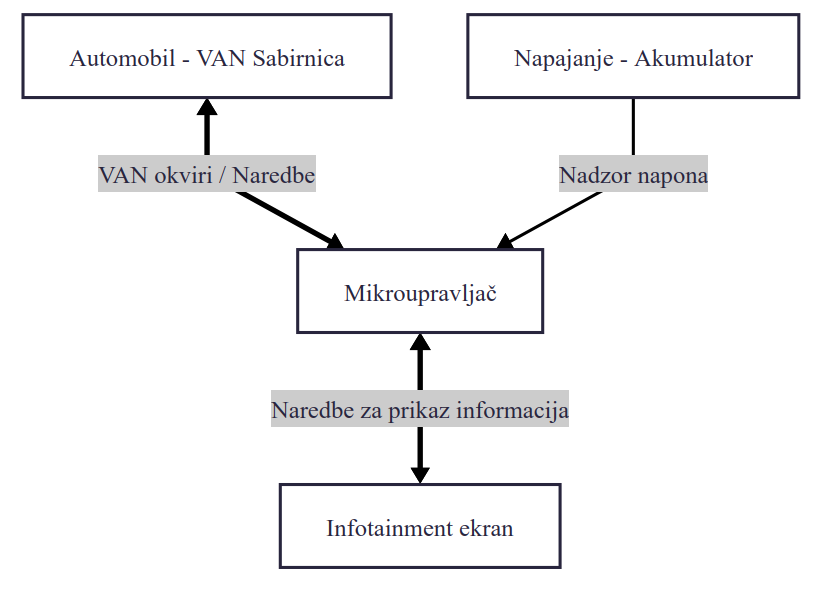
\includegraphics[width=0.75\textwidth]{images/block_diagram_2_3.png}
    \caption{Osnovni blok dijagram programskog rješenja}
    \label{fig:block_diagram_2_3}
  \end{center}
\end{figure}

